\documentclass{article}
\usepackage[utf8]{inputenc}
\usepackage{graphicx}
\usepackage{caption}
\usepackage{amsmath}
\usepackage{algorithm}
\usepackage[noend]{algpseudocode}
\usepackage[english]{babel}
\usepackage{natbib}

\title{Octave: A Generative Music Engine using Genetic Algorithms and Markov Matrices}
\author{Abhiram Kothapalli}
\date{}

\begin{document}

\maketitle

\begin{abstract}
We propose a novel generative music algorithm by genetically evolving order 1 Markov matrices that represent note transition probabilites. In order to make Markov matrices a suitable population element for a genetic algorithm we define new definitions of the genetic operators crossover and mutate. Additionally we define a robust yet efficient fitness function by combining a series of simple fitness functions based on simple musical rules. We implement our algorithm to show that it can create interesting melodies in an very efficient manner. We analyze the effect of different genetic parameters on the quality of the final composition.
\end{abstract}

\section{Introduction}

Generative music, namely music that is algorithmically composed, has been explored quite thoroughly by numerous different disiplanes. In the domain of machine learning past works have used recurrent neural networks for their advantages with time based learning \cite{akten9realtime, 938515, DBLP:journals/corr/Graves13}, genetic algorithms \cite{eigenfeldt2015generative, miranda2001composing}, and Markov matrices \cite{fernandez2013ai}. Despite numerous efforts algorithmically generated music still has not achieved the quality and creativity of human composers. This work, while it does not break new grounds in the quality of the output compositions, explores a fresh approach to creating music by using genetic algorithms to evolve Markov matrices representing note transition probabilities. The key insight lies in combining both Markov matrices and genetic algorithms to create a novel and unexplored approach to generative music. We are able to achieve this sort of combination by redefining the genetic operations and fitness functions found in genetic algorithms to fit Markov matrices as population elements.

\paragraph{Previous Work} The field of generative music is almost entirely dominated by recurrent neural networks in the machine learning domain. Solutions usually take some input musical string and attempt to learn the implicit patterns in note progression with varying degrees of success. Google's open source Magenta project \cite{weydeperception} which uses deep learning to generate artwork and music is perhaps the most up to date and robust recurrent neural network used for this end. While Magenta has been able to produce interesting compositions they are limited in length to around 30 seconds and requires a large dataset of input sequences. This makes generating tunes and melodies on the fly cumbersome. Genetic algoritms have also been explored my multiple works but are usually limited by a weak or unrefined fitness function. Some past genetic algorithms have suggested using the human ear as a fitness function \cite{miranda2001composing}. While this provides the highest quality measure of fitness it is not scalable and cannot function outside of trivial population sizes and iterations. Other fitness functions have attempted to use tonal rules \cite{matic2013genetic} but these are limited in scope and cannot control the quality of overall flow and rhythm. Finally Markov matrices are one of the oldest methods and simply study the most likely probability distribution over a large data set for the next note conditioned on a previous note \cite{fernandez2013ai}. While Markov matrices are simple and much faster to compute than recurrent neural networks they cannot keep track of past data very well and therefore do not produce very interesting compositions when used alone.

\paragraph{Contribution} We are the first to produce a novel combination of previous algorithms by evolving Markov matrices using genetic algorithms. This allows us to combine the speed and efficiency of generating Markov matrices with the probabilistic power of generative algorithms to select the most optimal matrix for a set of conditions. Unlike most works in the domain, our proposed algorithm does not use any seed training compositions. Instead we build our compositions from scratch using a robust fitness function using simple musical guidelines. Additionally we create an algorithm that is computationally simple to allow music to be generated cheaply and repeatedly.

\section{The Generative Algorithm}

The music composition algorithm works by genetically evolving Markov matrices that represent note transition probabilities.

\subsection{Markov Matrix Population Element}

The generative algorithm uses order 1 Markov matrices to represent note transition probabilities. Each row represents the previous note and the elements of that row represent probability distribution for the next note conditioned on the previous note. We also include a row and column to represent a pause. We can simulate the progression of notes using these probabilities to create a musical piece. Unlike standard genetic algorithms which evolve fixed segments of notes, this model allows us to define and evolve infinitely long musical pieces.

\paragraph{Order N Markov Matrices} We additionally explore the possibility of order N Markov matrices. In this context an N Order matrix represents the probability distribution conditioned on the last N notes. However an order $N$ Markov matrix requires $N^2$ rows making it computationally infeasible outside of some trivial $N$.

\subsection{Genetic Evolution Algorithm}

A genetic algorithm functions by repeatedly taking a population of candidates, selecting a subset of the population using some fitness function, and finally performing genetic operations such as crossover and mutate to create a new population. This process can be summarized as below:

\begin{enumerate}
\item Initalize: Randomly create a population by generating $N$ candidates
\item Select: Select an optimal subset of population $P_k$ by picking $S \subset P_k$ based on some fitness function $f(P_{ki})$
\item Genetic Operations
  \begin{enumerate}
  \item Crossover: Pick two elements $s_1, s_2 \in S$ such that elements with higher fitness have a higher probability of being picked. Merge these elements using some function $crossover(s_1, s_2)$ and place the output element in population $P_{k + 1}$.
  \item Mutate: Modify element $s \in P_{k + 1}$ with a small probability $\gamma$
  \end{enumerate}
\item Iterate: Continue iterating the population by repeating steps 2 and 3 until the population fitness converges.
\end{enumerate}

We redefine the genetic operations and fitness function to fit the constraints of Markov matrices as population elements.

\subsubsection{Genetic Operations on Matrices}

\paragraph{Crossover} While there are several approaches to merging two Markov matrices, We chose to merge $s_1$ and $s_2$ by picking a random split point, $j$, among the rows and copying rows above $j$ from $s_1$ and rows $j$ and below from $s_2$. Intuitively this means that we inherit the probability distributions for some notes from parent 1 and the distributions for the remaining notes from parent 2.

\begin{algorithm}[H]
  \caption{Crossover}
  \begin{algorithmic}
    \State Initalize randomly selected split point, j
    \State Initalize parents $s_1, s_2$
    \While{i $<$ number of rows}
    \If {$i < j$}
    \State $child_i \gets s_{1i}$
    \EndIf
    \If{$i \geq j$}
    \State $child_i \gets s_{2i}$
    \EndIf
    \State $i \gets i + 1$
    \EndWhile
    \State Return child  
  \end{algorithmic}
\end{algorithm}


\paragraph{Mutation} There are also several options for mutating matrices. We simply modify an element in the matrix with some set mutation probability, $\gamma$.

\begin{algorithm}[H]
  \caption{Mutation}
  \begin{algorithmic}
    \State Assume some $\gamma$ has been set

    \While{i $<$ number of rows}
    \While{j $<$ number of columns}
    \If{Probability $\gamma$ is satisfied}
    \State $matrix[i][j] \gets $ random new probability
    \EndIf
    \EndWhile
    \EndWhile
  \end{algorithmic}
\end{algorithm}


\subsubsection{Fitness Function on Matrices}

As with any genetic algorithm the fitness function is crucial to creating Markov matrices that represent satisfying music. In fact, creating an effective fitness function to judge musical compositions is an active area in research. In an attempt to preserve creativity and allow a wide variety of results, we aimed to create a simple yet effective fitness function. A simple fitness function essentially needs to capture and judge adherence to the fundamental rules of pleasing music. To achieve this end, we identify several key characteristics of pleasing music:

\begin{enumerate}
\item Ascending and descending note sequences
\item Occasional pauses
\item A balance between long and short notes
\item Unexpected jumps and variations
\end{enumerate}

Implementing these rules individually is easy. We can just give larger fitness scores to matrices that have transition probabilities adhering to these sorts of rules. However these rules when used individually as fitness functions lead to uninteresting and repetitive melodies, due to their simplicity. We can create more interesting rules by creating a new fitness score resulting in a weighted linear combination of simpler fitness scores. For example a more robust fitness function can value frequent pauses and unexpected jumps placing a higher emphasis on the latter.  This allows us to keep the overall simplicity of assessing the fitness of our matrices while still producing interesting compositions. If we have simplistic fitness functions $f_1, f_2, f_3, ..., f_k$ and weights $w_1, w_2, w_3, ..., w_k$ for these fitness functions, our robust fitness function, $f_r$, can be summarized with the following representation.

\[
f_r(m) = \sum_{i = 1}^k{w_i * f_i (m)}
\]

\section{Implementation and Evaluation}

We have created a working implementation of the proposed generative algorithm in order to experimentally evaluate the musical quality based on different parameters and fitness functions. The breakdown of the implementation can be described by its component files:

\begin{enumerate}
\item generator.py: Contains the genetic algorithm process. Takes in population element constructor, crossover, mutate and fitness function as an argument. Also takes in number of generations, number of elements per population and exclusivity function.
\item markov.py: Contains definitions for how to construct, crossover, and mutate a markov population element. Also contains the fitness function rule based on fitness.py
\item fitness.py: Contains various fitness functions that can be used and combined in markov.py
\item playmarkov.py: Generates a Markov matrix with specifications set in markov.py or takes an argument to an existing markov matrix. Plays the resulting Markov matrix.
\end{enumerate}

The projects source code and supporting files can be found at the following links. We can subjectively assess of the success of the proposed algorithm by listening to the provided sound samples.


\begin{itemize}
\item Source: https://github.com/abhiramkothapalli/Octave.
\item Sample Compositions: https://github.com/abhiramkothapalli/Octave/tree/master/samples.
\item Sample Matrices: https://github.com/abhiramkothapalli/Octave/tree/master/matrices
\end{itemize}

\subsection{Parameter Analysis}

\subsubsection{Varying Mutation Probability}

\begin{figure}[H]
\centering
\begin{minipage}{.5\textwidth}
  \centering
  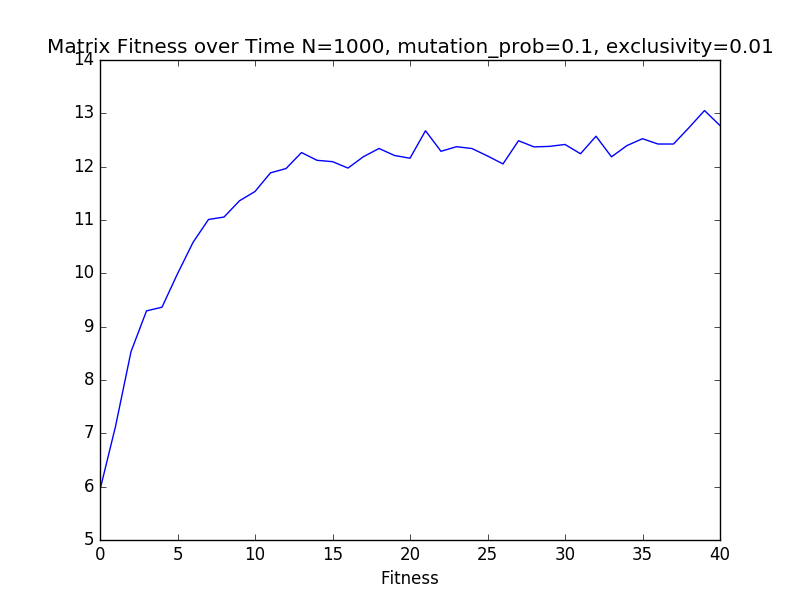
\includegraphics[width=1\linewidth]{../graphs/fitness1.png}
  \captionof{figure}{Mutation Probability 0.1}
\end{minipage}%
\begin{minipage}{.5\textwidth}
  \centering
  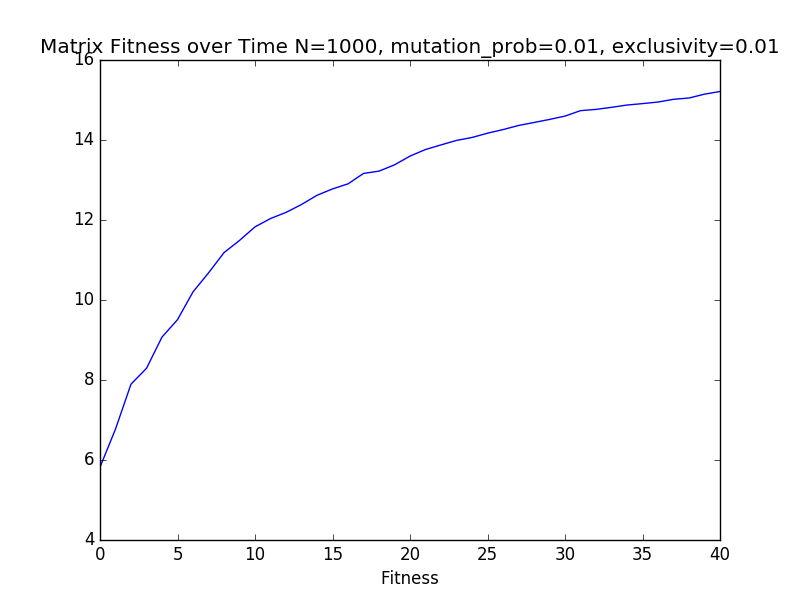
\includegraphics[width=1\linewidth]{../graphs/fitness2.png}
  \captionof{figure}{Mutation Probability 0.01}
\end{minipage}
\end{figure}

As seen in the figures above a reasonably small mutation probability converges more stably and converges to a higher population fitness. The second configuration is able to produce music that fits the prescribed rules better but does not necessarily sound better. This is a good example of how weak tuning, in fact, allows more space for creativity giving us more interesting compositions.

\subsubsection{Varying Population Size}

\begin{figure}[H]
\centering
\begin{minipage}{.5\textwidth}
  \centering
  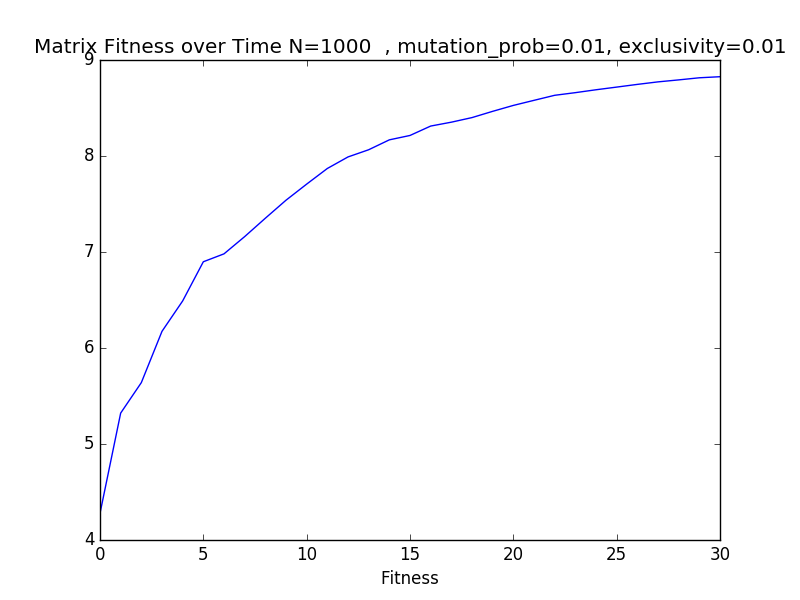
\includegraphics[width=1\linewidth]{../graphs/population1.png}
  \captionof{figure}{N = 1000}
\end{minipage}%
\begin{minipage}{.5\textwidth}
  \centering
  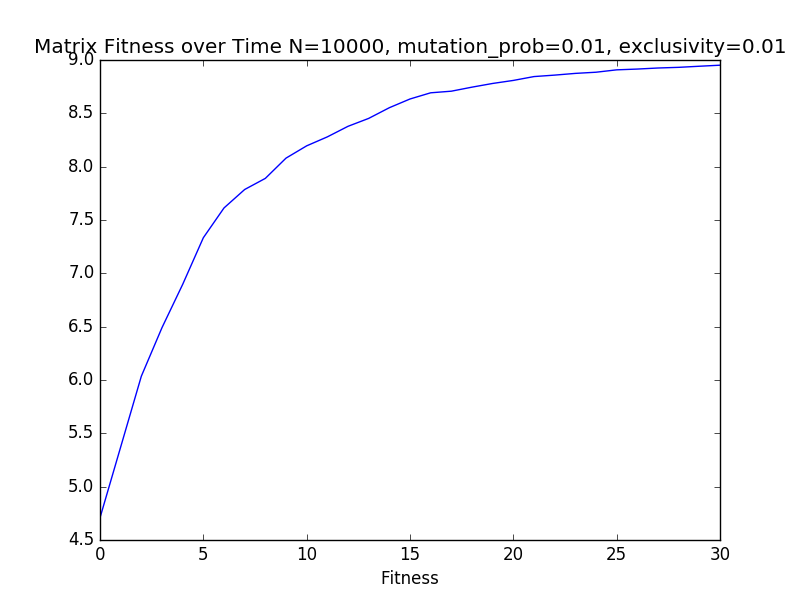
\includegraphics[width=1\linewidth]{../graphs/population2.png}
  \captionof{figure}{N = 10000}
\end{minipage}
\end{figure}

Upon close inspection we can tell that a population size of 10000 converges faster but both end up with the same fitness score. This show's that over time the number of population elements so long as it's reasonably high is insignificant. This implies that we can get fairly optimized compositions with only a relatively small population size. 

\section{Future Work}

Perhaps the most critical area of development is to create a stronger more robust fitness function. We could potentially use the same generative algorithm but experiment with an entirely new class of fitness function, perhaps one that attempts to follow the patterns from input examples. We can also use our genetic algorithm algorithm on any sort of population element so long as it is simple enough. In the fuure we can implement neural networks or decision trees as our population element so long as we can create reasonable genetic operations and fitness functions. We hope to refine this algorithm until musicians can start defining their own intuitive fitness functions and incorporate the output in their work.

\section{Conclusion}

In summary, we create a novel musical composition algorithm by genetically evolving Markov matrices. Because Markov matrices only contain the note transition probabilities we can train on and optimize infinite sequences of notes. In order to make Markov matrices compatible with a population element we define new genetic operators, crossover and mutate. Additionally we define a robust yet efficient fitness function by combining a series of simple fitness functions. This proved to be efficient but still capible of creating interesting melodies. We implement the discussed algorithm to prove that it can, in fact, create interesting melodies and to analyze the effects of different genetic parameters.


\bibliographystyle{plain}
\bibliography{final_report}

\end{document}



